\section{Diagram klas}
\subsection{Rysunek (diagram)}
\begin{figure}[!htb]
    \centering
    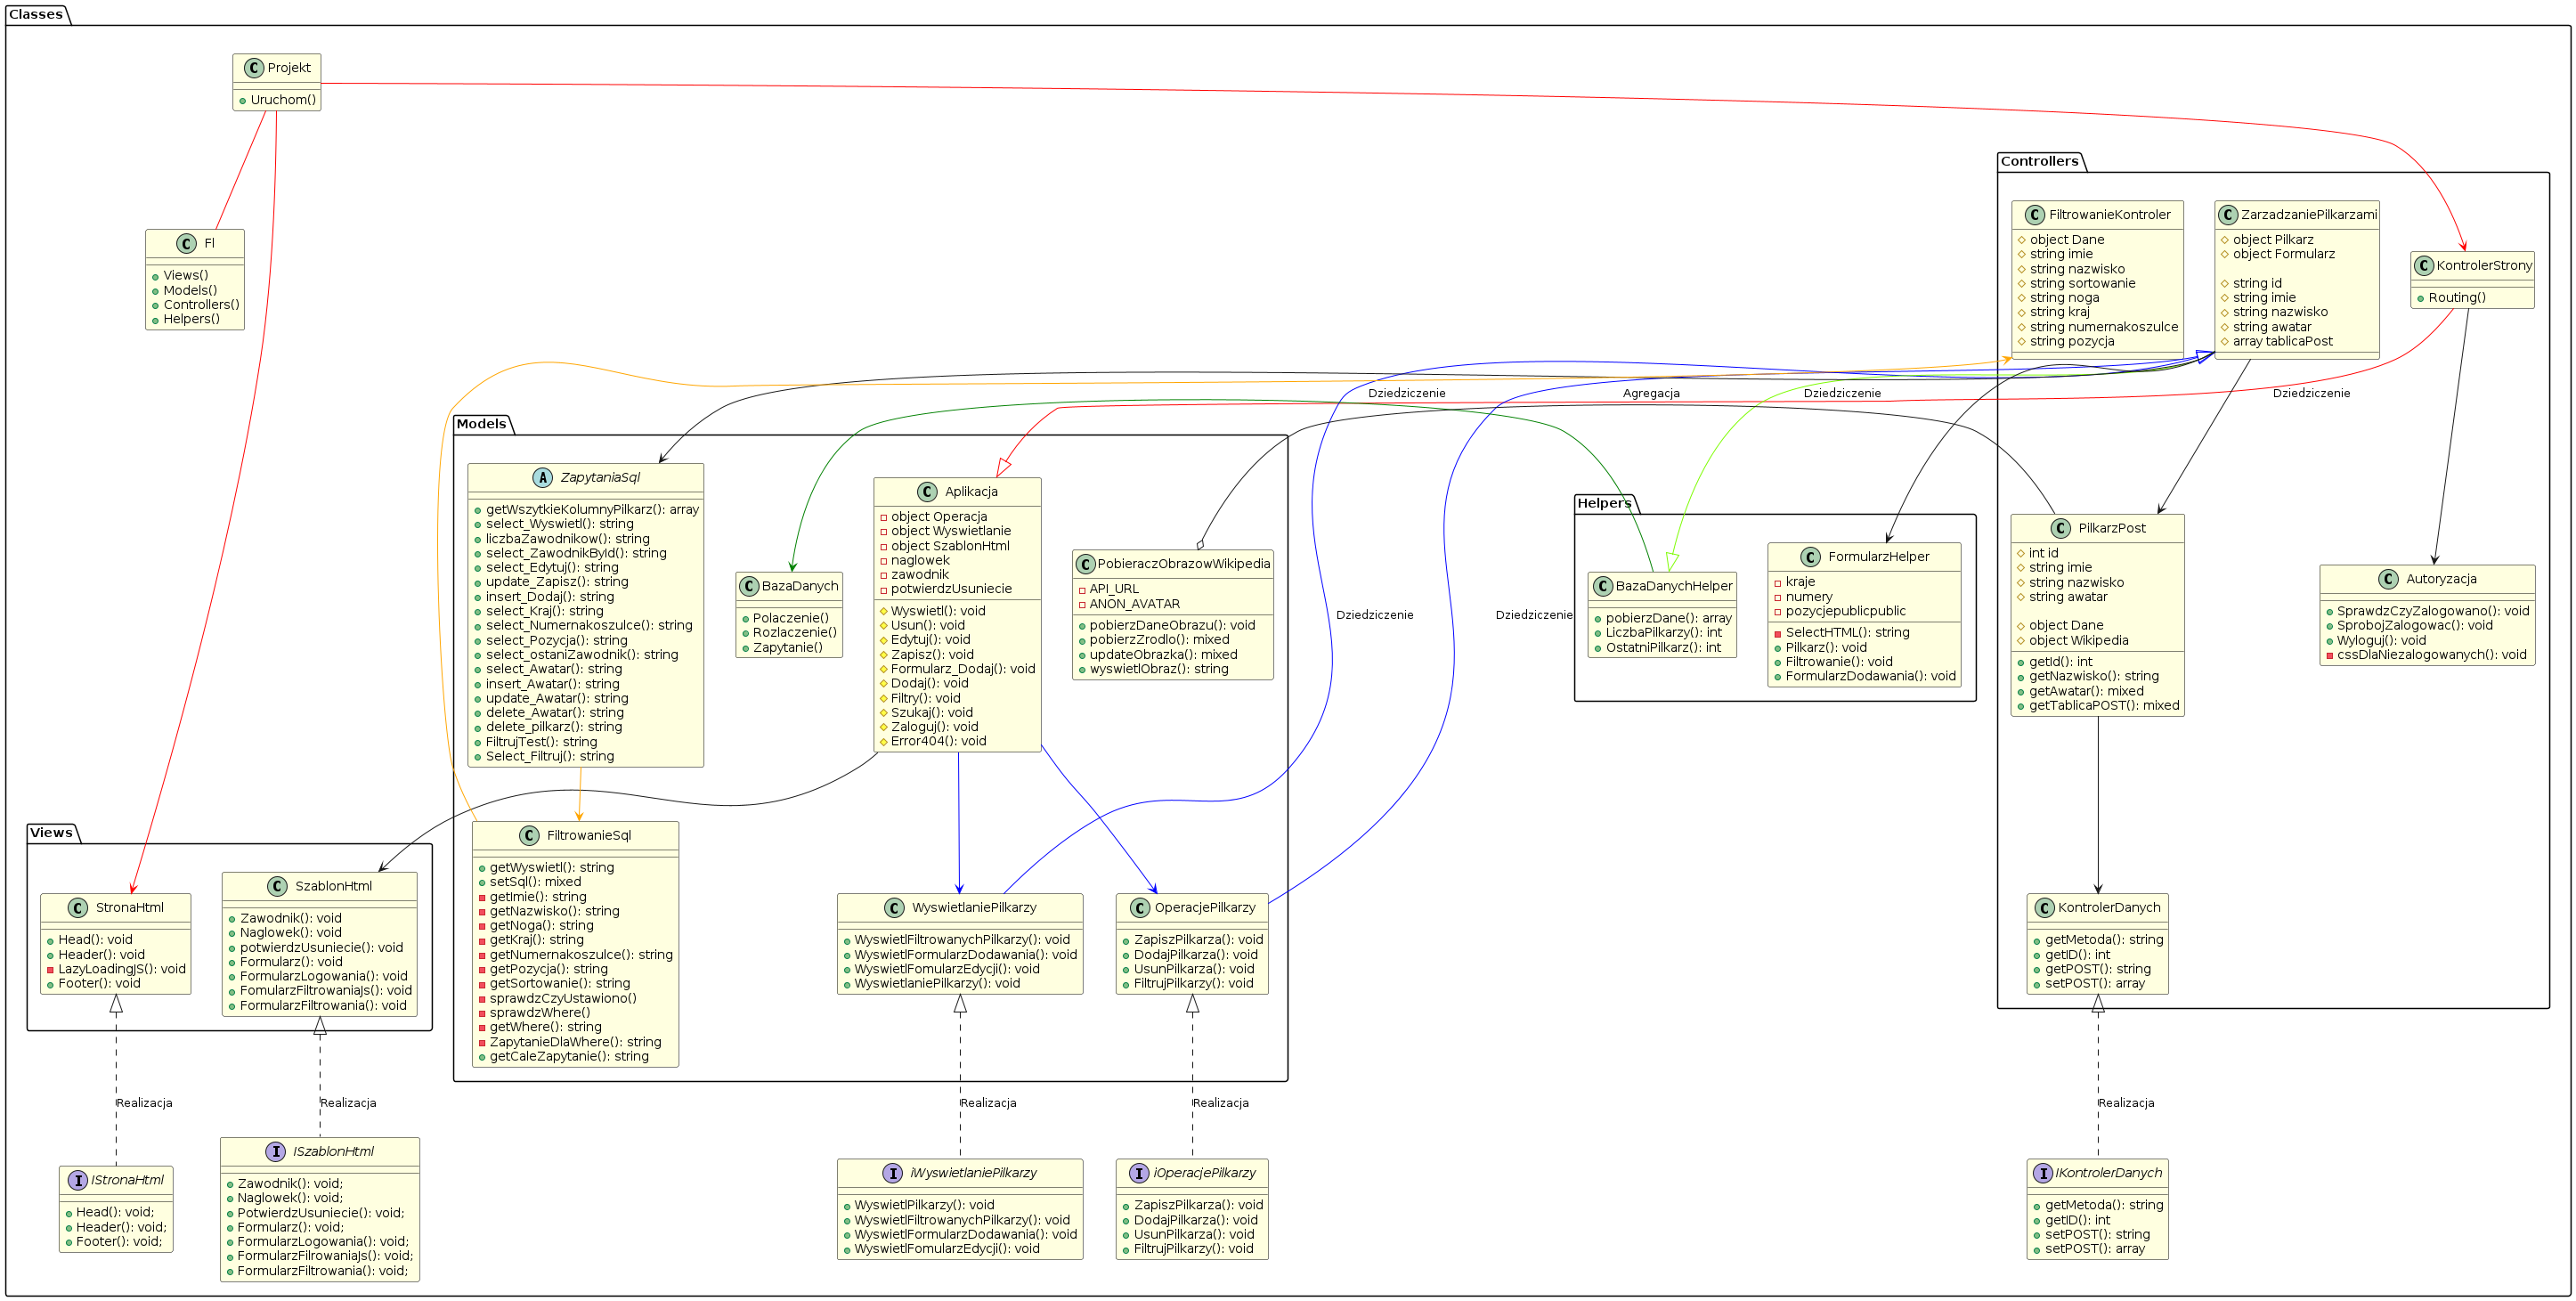
\includegraphics[width=1.0\textwidth]{diagramy/klas.png}
    \caption{Diagram klas}                
\end{figure}

\subsection{Opis przeznaczenia klas}
    Klasy są segregowane według modelu \textbf{MVC} i pomocniczych klas opisanych jako \textbf{Helpers}

\subsection{Models}
    \subsubsection{Aplikacja}
    Stanowi rdzeń całej struktury programu, zarządzając jego ogólnym działaniem, inicjalizacją, oraz kontrolą przepływu danych i interakcji między poszczególnymi komponentami. Jest to kluczowy element, który koordynuje i integruje funkcjonalność innych klas, tworząc spójną aplikację.
    Skupia się na zarządzaniu operacjami związanymi z piłkarzami w kontekście aplikacji. Posiada różne chronione metody , które współpracują z innymi klasami, takimi jak OperacjePilkarzy, WyswietlaniePilkarzy oraz SzablonHtml. Te metody wykonują różne zadania, takie jak wyświetlanie, usuwanie, edytowanie, dodawanie, filtrowanie oraz obsługę błędów w aplikacji związanych z piłkarzami. Klasa ta inicjuje obiekty innych klas w swoim konstruktorze i wykorzystuje je do odpowiedniego przetwarzania i wyświetlania danych w interfejsie użytkownika.

    \subsubsection{BazaDanych}
    Odpowiedzialna jest za obsługę połączenia z bazą danych, zarządzanie połączeniem  oraz zapewnienie ogólnej komunikacji z nią. Jest kluczowym połączeniem między aplikacją a danymi przechowywanymi w systemie.

    \subsubsection{ZapytaniaSql}
    Definiuje i obsługuje generowanie zapytań SQL do bazy danych. Odpowiada za tworzenie struktur zapytań, umożliwiając aplikacji komunikację z bazą w celu pobierania, aktualizacji, usuwania i wstawiania danych.

    \subsubsection{FiltrowanieSql}
    Jest odpowiedzialna za filtrowanie danych otrzymanych z bazy danych. Zapewnia mechanizmy filtrowania danych, aby  zwracać jedynie pożądane informacje w spójny sposób. Wynikiem końćowym metody \textit{getCaleZapytanie()} jest 
    jedno poprawne zapytanie SQL przekazane do wykonania do bazy danych.  

    \subsubsection{OperacjePilkarzy}
    Dostarcza zestaw operacji związanych z zarządzaniem danymi dotyczącymi piłkarzy w aplikacji. Obejmuje dodawanie, usuwanie, edycję danych piłkarzy oraz inne operacje z nimi związane.

    \subsubsection{WyswietlaniePilkarzy}
    Klasa koncentruje się na prezentacji danych dotyczących piłkarzy. Zapewnia funkcje prezentacji, sortowania, wyświetlania informacji o piłkarzach, dostosowanej do interfejsu użytkownika.

    \subsubsection{PobieraczObrazowWikipedia}
        Klasa za pomocą otwartego API Wikipedia, pobiera adres URL do głównego zdjęcia piłkarza z artykułu na Wikipedii. Zdjęcie jest pobierane podczas dodawania nowego piłkarza bądź jego edycji i zapisywana w bazie danych w tabeli \textbf{awatar} w postaci linku.

    \subsection{Controllers}
        \subsubsection{Autoryzacja}
        Obsługuje mechanizm uwierzytelniania użytkowników. Wykorzystuje wbudowany mechanizm sesji w PHP do uwierzytelniania, zapewniając kontrolę dostępu i identyfikację użytkowników w aplikacji.

        \subsubsection{FiltrowanieKontroler}
        Odpowiada za filtrowanie danych otrzymywanych od użytkownika. Jest odpowiedzialna za proces sprawdzania, walidacji i filtrowania danych wejściowych (takich jak parametry GET z adresu URL oraz dane POST z formularzy), aby zapewnić bezpieczeństwo i poprawność przetwarzanych informacji.


        \subsubsection{KontrolerDanych}
        Ta klasa ma na celu odbieranie danych od użytkownika z poziomu aplikacji, korzystając z metod GET (parametry z linku) i POST (dane przesyłane z formularzy). Zarządza odbiorem, przetwarzaniem i kontrolą danych, zapewniając ich poprawność i integrację z aplikacją.

        \subsubsection{PilkarzPost}
        Zajmuje się operacjami na danych związanych z piłkarzami, odbierając i przetwarzając informacje przesłane od użytkownika z formularzy POST. Realizuje operacje zapisu danych związanego z piłkarzami do systemu.

        \subsubsection{ZarzadzaniePilkarzami}
        Jest klasą, która wykorzystuje klasę pomocniczą BazaDanychHelper do operacji na bazie danych w kontekście informacji o piłkarzach. Ta klasa definiuje podstawowe funkcje i metody obsługi informacji o piłkarzach, wykorzystując metody HTTP - GET i POST do pobierania oraz przesyłania danych.

    \subsection{Views}
        Views (pol. Widoki), ta sekcja zawiera metody, które reprezentują wartwę graficzną aplikacji w HTML, CSS i JavaScript. Odpowiada za poprawne wyświetlanie informacji, które zostały uzyskane z bazy danych.
        \subsubsection{StronaHtml}
        Zawiera szkielet strony HTML, taki jak sekcja <head> <body> <footer> czy <header>. Dzięki temu rozwiązaniu można ustawić Podstawowe dane takie jak tytuł strony, autorów, w kiklu miejscach na stronie, wczytywana z pliku konfiguracyjnego \textbf{KonfiguracjaApp.php}


        \subsubsection{SzablonHtml}
        Klasa zawiera komponenty HTML, które służą do wyświetlania elementów, takich jak card (karta z informacją o piłkrzu), formularze, panel logowania.

    \subsection{Helpers}

        \subsubsection{BazaDanychHelper}
        Służy do udostępniania metod wspomagających operacje bazodanowe, takie jak łączenie się z bazą danych, wykonywanie zapytań czy inne operacje związane z bazą danych. 

        \subsubsection{FormularzHelper}
        Zawiera metody pomocnicze związane z tworzeniem, walidacją czy obsługą formularzy w aplikacji.

        
    \subsection{Projekt}
    Klasa ta jest ostatecznym elementem programu, posiadającym metodę \textit{Uruchom()}, która integruje Routing, StronęHtml oraz klasę Aplikacja w celu właściwego uruchomienia programu z zachowaniem odpowiedniej kolejności działań. Metoda \textit{Uruchom()} łączy te elementy w logiczną sekwencję, umożliwiając kompleksowe działanie aplikacji poprzez współpracę wymienionych składników w spójny sposób.

    \lstinputlisting{./src/code_snippets/oop-php/classes/Projekt.php}  

    \subsection{FileLoader}    
    Klasa ma jedynie jedno przeznaczenie: załączenie plików z klasami do projektu. Jej rola polega na importowaniu (łączeniu) różnych plików zawierających klasy, co umożliwia poprawne funkcjonowanie projektu poprzez dostęp do niezbędnych klas i ich metod.
    \lstinputlisting{./src/code_snippets/oop-php/classes/FileLoader.php}  


    \subsection{plik - index.php}    
    Ten plik inicjuje metodę \textit{Uruchom()} oraz wykorzystuje klasę FileLoader (skrót Fl) do załączenia plików. Jego głównym zadaniem jest uruchomienie metody \textit{Uruchom()} oraz korzystanie z klasy FileLoader w celu załadowania plików do projektu.
    \lstinputlisting{./src/code_snippets/oop-php/index.php}  